\documentclass[a4paper]{paper} 
%\usepackage{babel}
\usepackage{hyperref}
\usepackage{amsfonts}
\usepackage{amsmath}
\usepackage{graphicx}
\usepackage[space]{grffile}
\usepackage[margin=2.5cm]{geometry}
\usepackage{pdfpages}
%\usepackage{graphicx}
\usepackage[capitalize,noabbrev]{cleveref}

\DeclareMathOperator*{\argmax}{arg\,max}

\graphicspath{{img/}}
\title{Improve path finding in the Lightning Network with the Health Improvement Algorithm}
\subtitle{Draft version}
\author{Rene Pickhardt} 
\institution{NTNU Gjovik} 

\begin{document} 
\twocolumn[\maketitle 
\hrule 
\begin{abstract}
  Making a payment in privacy aware payment channel networks is currently achieved by trying several payment paths until one succeeds which can yield to several minutes for a payment to complete.
  We introduce a health measure for the lightning network and provide emperical evidence that a better health of the network leads to higher a success rate for making a random payment.
  We formulate the optimization problem of improving the health of the network as a sequence of rebalancing operations of the funds within the channels along circular paths within the network.
  As the funds and balances of channels are not globally known we introduce a greedy heuristic with which every node despite the uncertainty can improve its own health.
  Since the health of the network is defined as the average of the health of its participants the network health will be improved if any participant improves its own health. 
  We also suggest to allow channel partners to share information with each other which can be probed anyway and engage in fee free rebalancing operations if that operation is benefitial for the health of every participant along the rebalancing circle.
  In this way participants will only be able to improve their health if this operation does not worsen the health of other nodes making sure that the heuristic will always improve the health of the network.
  We show emperically on synthetic random networks that the health measure is well defined and that our greedy heuristic quickly converges into a healthy enough network that supports random payments without failures.
\end{abstract}

\begin{keywords}
Optimization, convex optimization, Bitcoin, Lightning Network, payment channel networks, path finding, routing, liquidity, flow control, congestion control, game theory, uncertainty, simulations, agent based systems, collaborative problem solving, 
\end{keywords}
\hrule\bigskip
]


%==========================================================================
\section{Introduction}
Payment channel networks have been introduced to mitigate the scaling issues of blockchain technologies such as Bitcoin\cite{poon2016bitcoin}.
With the help of smart contracts payment channels are created that allow the cryptographically secure transfer of value without the necessity to record the transaction to the central ledger.
This yields new and interesting privacy properties for the participants of the network.
In order to protect the privacy while routing a payment through several payment channels privacy aware payment cannel networks use a source based onion routing scheme like the Sphinx Mix format \cite{danezis2009sphinx}.
This prevents routing nodes from learning who paid whom.

While the lightning network for example shares the capacity of public channels with its participants through its gossip protocol the local split of the capacity of the channels into the balance of its participants is not being shared with the rest of the network for two reasons:
First this would compromise the privacy as one could collect all changes of the channel balances and reconstruct the flow of payments.
Second propagating this information would essentially mean that every node in the network is made aware of every payment which would have the same poor scaling properties as blockchain technologies.
The decision to use source base routing together with the unknown channel balances of the network results in a challange for finding a path of payment channels that have enough balance to be able to route an attempted payment.
Currently this challange is met by probing paths until one is found in which each channel has enough balance to forward the payment.
It has been shown that probing for paths can take more than 3 minutes in more than $5\%$ of the attempted payments \cite{decker2019lnconf} which leads to a poor user experience.
Imagine a grocery store in which for every 20th customer the cashregister would have to wait three minutes until the payment was received.

In this paper we examine the idea of nodes proactively and collaboratively distributing their funds evenly accross their channels.
We introduce the notation of an imbalanced network.
The imbalance is measured as the average of the imbalance scores of its nodes.
The node's imbalance of payment channels as the gini coefficient of a node's channel balance coefficients which are the relative amount of funds a node owns in a channel in comparison to the capacity of that channel.
In particular nodes already have all the information they need to compute their imbalance. 
Nodes can reduce their imbalance either alone or collaboratively with the help of its channel partners by conducting circulare payments which is also known as rebalancing.

We formulate an optimization problem of finding a squence of rebalance operation that minimizes the networks imbalance.
As the information necessary to solve the optimization problem is not publically known in privacy aware payment channel networks we provide a greedy privacy aware agent based heuristic for its participants to find a minimum for the problem. 
In an empirical study we show that the greedy heuristic will lead to a $100\%$ successrate for an arbitrary payment to succeed.
We show that this is always the case if the balance of the network is good enough meaning that the imbalance score is low enough.
In particular we see that participants do not have to follow a strategy of having as much inbound capacity as outbound capacity for this algorithm to work. 

While single nodes can already execute the algorithm in currently existing payment channel networks they are economically disincentiviced to do so.
We thus discuss the possability to introduce fee free rebalancing and for the sake of speed we suggest that nodes share with their neighbors on which local channels they would like to have inbound or outbound capacity. 

The remainder of this paper is organized as follows in section \cref{sec:relatedWork} we give a short overview of related work in this field.
We then introduce the notation and definition of the imbalance score in section \cref{sec:formalization}.
After we show a small example of our definitions in section \cref{sec:example} we formulate the optimization problem to reduce the imbalance and propose a greedy, agent based and collaborative algorithm in \ref{sec:Algorithm} to address the optimization problem.
To improve the computational overhead of the algorithm we propose a few changes to the lightning network protocol in section \ref{sec:lnchanges}.
In \cref{sec:setup} we introduce the experimental setup and the data set that we used.
After showing our empirical results in \cref{sec:results} we discuss the results and propose some future work in the last two sections.



%==========================================================================
\section{Related Work}
\label{sec:relatedWork}

While the Lightning Network White paper~\cite{poon2016bitcoin} does not discuss path finding and states routing as an easy problem it is generally recognized that pathfinding on the lightning network is a difficult problem \cite{piatkivskyi2018split}, \cite{prihodko2016flare}, \cite{bagaria2019boomerang}, \cite{pickhardt2019pathfinding}, \cite{grunspan2018ant}, \cite{sivaraman2018routing}.
There is already research being conducted in the field of rebalancing channels~\cite{khalil2017revive} which was more about the cryptographic protocols used to make sure that participants can enforcethe rebalancing that was agreed upon.
There are rebalancing operations for c-lightning\footnote{\url{https://github.com/lightningd/plugins/tree/master/rebalance}} and for lnd\footnote{\url{https://github.com/bitromortac/lndmanage}}.
In particular the idea of Just in time rebalancing while fulfilling routing requests~\cite{pickhardt2019jit} is already being implemented for c-lightning\footnote{\url{https://github.com/lightningd/plugins/pull/66}}. 

\textbf{TODO:} Add statistical papers of the lightning network. Payment reliability and path finding methods (similar to PhD Proposal)


% ===========================================================================
\section{Formalization and Assumptions}
\label{sec:formalization}

Let $G=(N,E,c)$ be a privacy aware payment channel network with a finit set of nodes.
The payment channels are the edges in the network such that $E\subset N\times N$.
Additionally we have a publicly known capacity function $c: E\longrightarrow \mathbb{N}$ that assigns a capacity to every edge of the network.
For every edge $e=(u,v)$ we denote $e_u:=(e,u)$ as the first participant of the channel and $e_v=(e,v)$ as the second participant.
Every node can be assigned its set of channels which we encode with the neighbor function $n : N \longrightarrow 2^{E}$.
Similarly, if we want to denote the set of neighboring nodes we use the function $n_n : N \longrightarrow 2^{N}$.
Naturally, the capacity of every channel $e=(u,v)$ is privately split into the local balances with the balance function $b: E\times N\longrightarrow\mathbb{N}$ such that $b(e_u)+b(e_v)\stackrel{!}{=}c(e)$.

We define the channel balance coefficient for $u$ on the channel $e=(u,v)$ as  $\zeta_{(u,v)} = \frac{b(e_u)}{c(e)}$.
This is just a relative amount of funds that the participant $u$ has in the channel $e$.
Note since $b(e_u)+b(e_v)\stackrel{!}{=}c(e)$ we also have $\zeta_{(u,v)} + \zeta_{(v,u)}=1$

To make the following formulas easier to read let us introduce $U:=n_n(u)$ the denote a set of channel partners of participant $u$.
The total funds of a participant $u$ are denoted as $\tau_u:=\displaystyle{\sum_{e\in U}b(e_u)}$.
The value of $\tau_u$ is constant while the balance function $b$ can vary subject to re-allocation of funds.
Similarly the total capacity of a participant $u$ is denoted as $\kappa_u:=\displaystyle{\sum_{e\in U}c(u)}$.
Using the last two definitions let us define the node balance coefficient for a participant $u$ as $\nu_u = \frac{\tau_u}{\kappa_u}$.

Let us call a node $u$ {\bf balanced} if its channel balance coefficients $\zeta_{(u,v_1),\dots,\zeta_{(u,v_d)}}$ have the same value.
This means that the relative distribution of a nodes funds across all its channels is the same.
Consequently, we consider a node {\bf imbalanced}, if it local channel balance coefficients are unequal.
Statistically, inequality of a distribution can be measured with the Gini coefficient.
Thus, for a node $u$ with channel balance coefficients $\zeta_{(u,v_1),\dots,\zeta_{(u,v_d)}}$ we define $G_u = \frac{\displaystyle{\sum_{i\in U} \sum_{j \in U}} | \zeta_i - \zeta_j |}{2 \displaystyle{\sum_{i \in U} \sum_{j \in U} \zeta_j}}$
If $G_u = 0$ this means that the channel balance coefficents are equal.
In contrast, if $G_u = 1$ the channel balance coefficients are distributed in the most unequal way.

Note, that the Gini coefficient of a channel balance coefficients of a node $u$ takes the value $0$ if and only if its channel balance coefficents all take the same value.
This value will be exactly the same as the node's balance coefficient $\zeta_u$.

Finally, $G$ denotes the imbalance of the network. $G = \displaystyle{\frac{1}{|N|}\sum_{n\in N}G_n}$. Imbalance $G$ is the mean of the imbalance values of all nodes in the network.
A perfectly balanced network would be achieved if $G$ takes the value of $0$ where as the balance is poor if the value of $G$ is close to 1.

Our goal is to find a balance function $b$ which minimizes $G$ given a privacy aware payment channel network with initial distribution of funds $\tau_{u_1},\dots,\tau_{u_n}$.
The constraint to this optimization problem that the total funds $\tau_u$ are fixed for every node $u \in N$ and any choice of the balance function $b$.
In a privacy aware payment channel network the distribution of funds $\tau_{u_1}\dots,\tau_{u_n}$ is not publicly known.\footnote{The initial distribution could be guessed from the funding transactions in the case of the Bitcoin Lightning Network for public channels. Note, this distribution will change with the first payment that is not a rebalancing operation.}
In the same way the initial balance function is not publicly known.
As we lack knowledge about the global network state, we cannot apply standard optimization techniques such as gradient descent, conjugate gradient methods or simulated annealing.
We suggest to use an agent based heuristic in which every participant executes some operations to improve its own help which others support if it also improves their health.
In the following subsection we describe a short example using the newly defined terminology. In the subsequent subsection we describe our rebalancing algorithm.


\subsection{Example}
\label{sec:example}

\begin{figure}
 \centering
 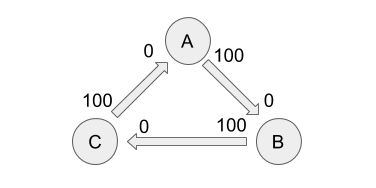
\includegraphics[width=8cm]{img/evenUnbalanced.png}
 \caption{A, B and C all own 100 satoshi.}
 \label{fig:evenUnbalanced}
\end{figure}

\cref{fig:evenUnbalanced} depicts a small network consisting of $3$ nodes in which the balances are distributed unevenly.
The global balance coefficient for every node is $\nu_u=0.5$.
The $\zeta$ values for each node are $0$ for the channel in which the node owns no funds and $1$ for the channel in which the node owns all the funds.
This leads to a local imbalance for every node of $0.5$. The global imbalance of the network $G$ is $0.5$.

\begin{figure}
 \centering
 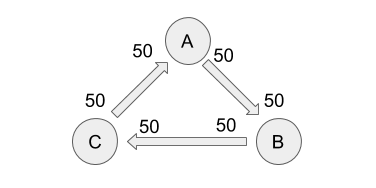
\includegraphics[width=8cm]{img/evenBalanced.png}
 \caption{Each node still owns 100 satoshi but distributed evenly balanced amonth their channels}
 \label{fig:evenBalanced}
\end{figure}

\cref{fig:evenBalanced} depicts a balanced view of this network.
The total funds $\tau_u$ stayed constant.
However, since the funds have been rebalanced the local balance coefficients $\zeta$ of every channel now take the value of $0.5$ leading to a local imbalance coefficient $G_u=0$ for every node $u\in N$.
This in turn leads to a perfectly balanced network with $G=0$.

Considering multi path payments in both cases of the network every node was able to pay the full funds they owned to every other participant.
If the edge $e=(A,B)$ was removed in the balanced network $A$ would still be able to pay $B$ with a path over $C$.
This would not be possible in the imbalanced network as the funds where distributed poorly.
It is worthwhile to mention that not every network can achieve a perfect global balance $G=0$.

\begin{figure}
 \centering
 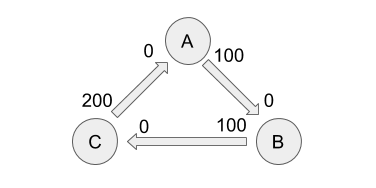
\includegraphics[width=8cm]{img/oddUnbalanced.png}
 \caption{Example of an unbalanced network that does not allow for perfect balance as funds are not distributed evenly.}
 \label{fig:oddUnbalanced}
\end{figure}

For example, \cref{fig:oddUnbalanced} depicts a case where perfect balance, with $G$ equal to $0$  is not possible. 
This is due to the fact that the funds are not distributed evenly among nodes -- node $D$ owns twice as many funds as the others.

\begin{figure}
 \centering
 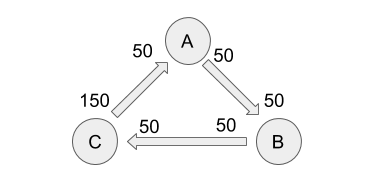
\includegraphics[width=8cm]{img/oddBalanced.png}
 \caption{Best possible balance in a network for which the funds are not distributed equally.}
 \label{fig:oddBalanced}
\end{figure}



\subsection{Description of the rebalancing algorithm}
\label{sec:Algorithm}

The developed rebalancing algorithm uses an agent-based heuristic in which participants can use the local knowledge and make local adjustments that result in a global convergence towards an improved overal netowrk balance. 
The algorithm solves the global optimization problem of finding $b$ such that the balance of the network is improved.

\begin{enumerate}
\item A node $u$ will compute its node balance coefficient $\nu_u$.
\item $u$ will then compute the channel balance coefficients $\zeta_{(u,v_1)},\dots,\zeta_{(u,v_d)}$ for its $d$ channels.
\item The node will select all channels $e=(u,v_i)$ for which its channel balance coefficient is higher than its node balance coeffient i.e $C = \{(u,v_i) | \zeta_{(u,v_i)} - \nu_u\ > 0\}$.\footnote{Note that we do not need to take absolute values as $u$ will only be able to initiate a rebalancing operation by sending money which means decreasing its cannel balance coefficient of $\zeta_{(u,v_i)}$}.
\item from the candidate set $C$ a random channel $e=(u,v)$ is selected.\footnote{We show in the experimental evaluation that always taking the channel with the biggest gain makes the heuristic stuck too quickly. The reason is that if a channel cannot be rebalanced in the next step the same channel is tried again.} 
\item Now the node searches for a circular payment to itself along $e=(u,v)$ by choosing a path $p = [u,v,x_1,\dots,x_n,u$. The amount of that payment should decrese the value of $\zeta_{(u,v)}$ to that of $\nu_u$ and can be computed as $a = c(e)\cdot (\zeta_{(u,v)}-\nu_u)$. Also the end of the circle should be a channel $(u,x_n)$ for which the channel balance coefficient $\zeta_{(u,x_n)}$ is smaller than the node balance coefficient $\nu_u$.
\item the node will conduct the payment if the nodes on the path $p$ agree to do this payment. 
 \item Repeat all steps as long as the local balance coefficients are still not even.
\end{enumerate}

In case a circular path exist it is easy to see that the making a payment along this path will make the distribution of local balance coefficients for node $u$ more even.
If no such circle can be found the local health is staying constant.
Obviously finding a circular rebalancing path is tricky as the balances of the network are not known and this will again boil down to probing as it is done currently in the lightning network for regular payments..
Also rebalancing might worsen the health of another node along the path in in that way not actually contributing to improve the global health.
The biggest drawback is that in the current implementation of the Lightning Network such a circular payment will cost the initator some routing fee which economically deincentivizes the node to improve its health even though our evaluation suggest that it will be benefitial for the network.

\subsubsection{Adoptions to the communication protocol}\label{sec:lnchanges}
In order to get rid of these problems we suggest to extend the communication protocol between channel partners and to update the algorithm.
.We take the idea of cost free rebalancing in the friend of a friend network as it was first proposed in the context of JIT-Routing \cite{pickhardt2019jit}.
In order to calculate a circular path node $u$ will query $v$ for the channels on which $v$ would be willing to forward the amount $a$ in a circular way.
$v$ will only return channels potentially with a lower amount than $x$ on which it  would also improove its local health $G_{v}$.
In the same way $u$ will ask the nodes though which channels it would like to receive the funds on which channels they would like to receive funds in a circular way to improve their health.
Both querries will allow the nodes to signal that they will be willing to participate in a rebalancing operation for up to $x$ tokens.
After the node $u$ has aquired this subset of channels in its friend of a friend network it searches for a path from $v$ to $u$.
This path will be preceeded with the first hop from $u$ to $v$ making it a circular payment.
The amount send on this circular payment will be the highest possible value up to $x$
Nodes will drop the routing fees for this circular path as it will improve the health of each node and provie a direct benefite instead of a routing service.

From a privacy point of view revealing channels on which a node is willing to participate in a rebalance operation to its neighbors does not directly leak more information than could be probed anyway.
Also nodes don't have to answer to the queries truethfully and could always intrudize some fuzziness for privacy reasons. 
While we suggest that channel partners share some information with each other this is not necessary for the algorithm to work.
First of all nodes can probe for rebalancing circles that are benifitial for itself.
Second s nodes on the way would only fulfill the fee free rebalncing request if it also improves their health this algorithm could work without actively sharing information in the friend of a friend network.

\section{Experimental Setup}\label{sec:setup}
We then conduct a simulation of the algorithm in the following way:
\begin{enumerate}
\item Assign $C$ as the candidate set of all nodes in the network.
\item As long as $|C| > 0$ do the following steps.
\item A random node from $C$ is chosen and is allowed to do one rebalancing operation to improve its network health executing the steps discussed in section \ref{sec:Algorithm}.
\item If the node was successfull go back to step $1$.
\item If the node could not improve its health remove the node from $C$ and go to step $3$.
\end{enumerate}
After each step we track all channel balance coefficients, local helth of nodes and the health of the network.

Comuting the rebalancing circles is the most expensive operation as a shortest path problem needs to be solved.
If the greedy heuristic is implemented in a real payment channel network this is not too expensive for a node as the shortest paths only need to be computed in a subset of the the friend of a friend network which is usually small enough to have no runtime issues.
Also in a real payment channel network this computation would only have to be conducted if the distribution of channel balance coefficents becomes too uneven which is cheaply monitored after every payment or routing attemtp.
However in the simulation the path finding operations add up so that we had to limit ourselves to rather small test networks.
We conducted our experiments on 3 graphs.
First a random network with $101$ nodes and $1788$ edges.
In order to have a larger diameter we did the experiments also on a random network with $1000$ nodes and $FILLOUT$ edges.
The capacity of nodes in these random networks are assigned a random value between $1000$ and $10000$ drawn from a uniform distribution.
Both random networks used the Erdos Renyi random network generator.
Finally to make it more realistic we conducted the experiment on the oldest existing lightning network channels which formed a strongly connected component to have a realistic network of $816$ and $7110$ edges.
The diameter of this network was 5 with the over a third of all pahts needing 4 or more hops.
In all three networks we assumed an initial distribution of the balances as the total capacity on one side of the channel.

% ==========================================================
\section{Results}\label{sec:results}

\begin{figure}
 \centering
 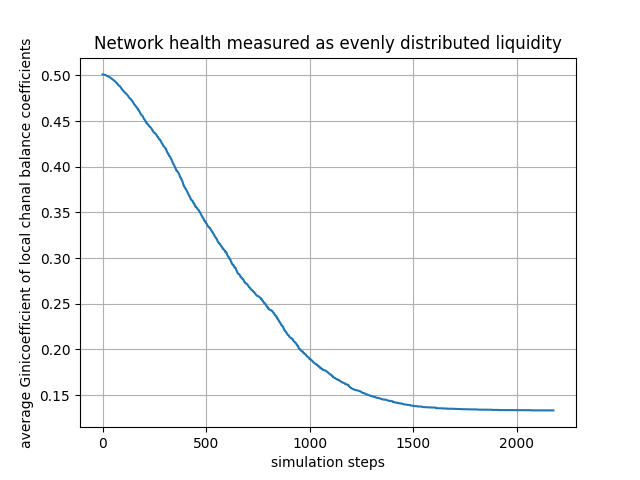
\includegraphics[width=7cm]{code/results/routabilityTest/1574847007_figure.png}
 \caption{Health evolving with execution of the algorithm on a network with 101 nodes and 1788 edges. The edges have been initialised with uniformly distributed capacities between $1000$ and $10000$ satoshi. Ihe full capacity is initially with the funder of the channel.}
 \label{fig:healthovertime}
\end{figure}

\cref{fig:healthovertime} confirms that the health score of the network is decreasing over time when running our simulation.
This means that the network is becoming more balanced or healthier.
We see that most improvement is happening quite fast with a few simulation steps.
On average, each node had attempted to rebalance at least $n$ times, where $n$ is the count of the node's payment channels.
This seams plausible in the sense that every channel gets rebalanced at least once.\footnote{Note that due to the collaborative behaviour of nodes a node also gets channel rebalanced in the rebalancing attempts of other nodes.} 
In particular the algorithm converges in a local minimum rather quickly.
Note, that the established minimum is a local minimum. 
Our experimental runs resulted in states that are not identical, however, the differences were negligible. 
We can therefore assume that the local minimum might be close to global minimum as the collected data demonstrate.

\begin{figure}
 \centering
 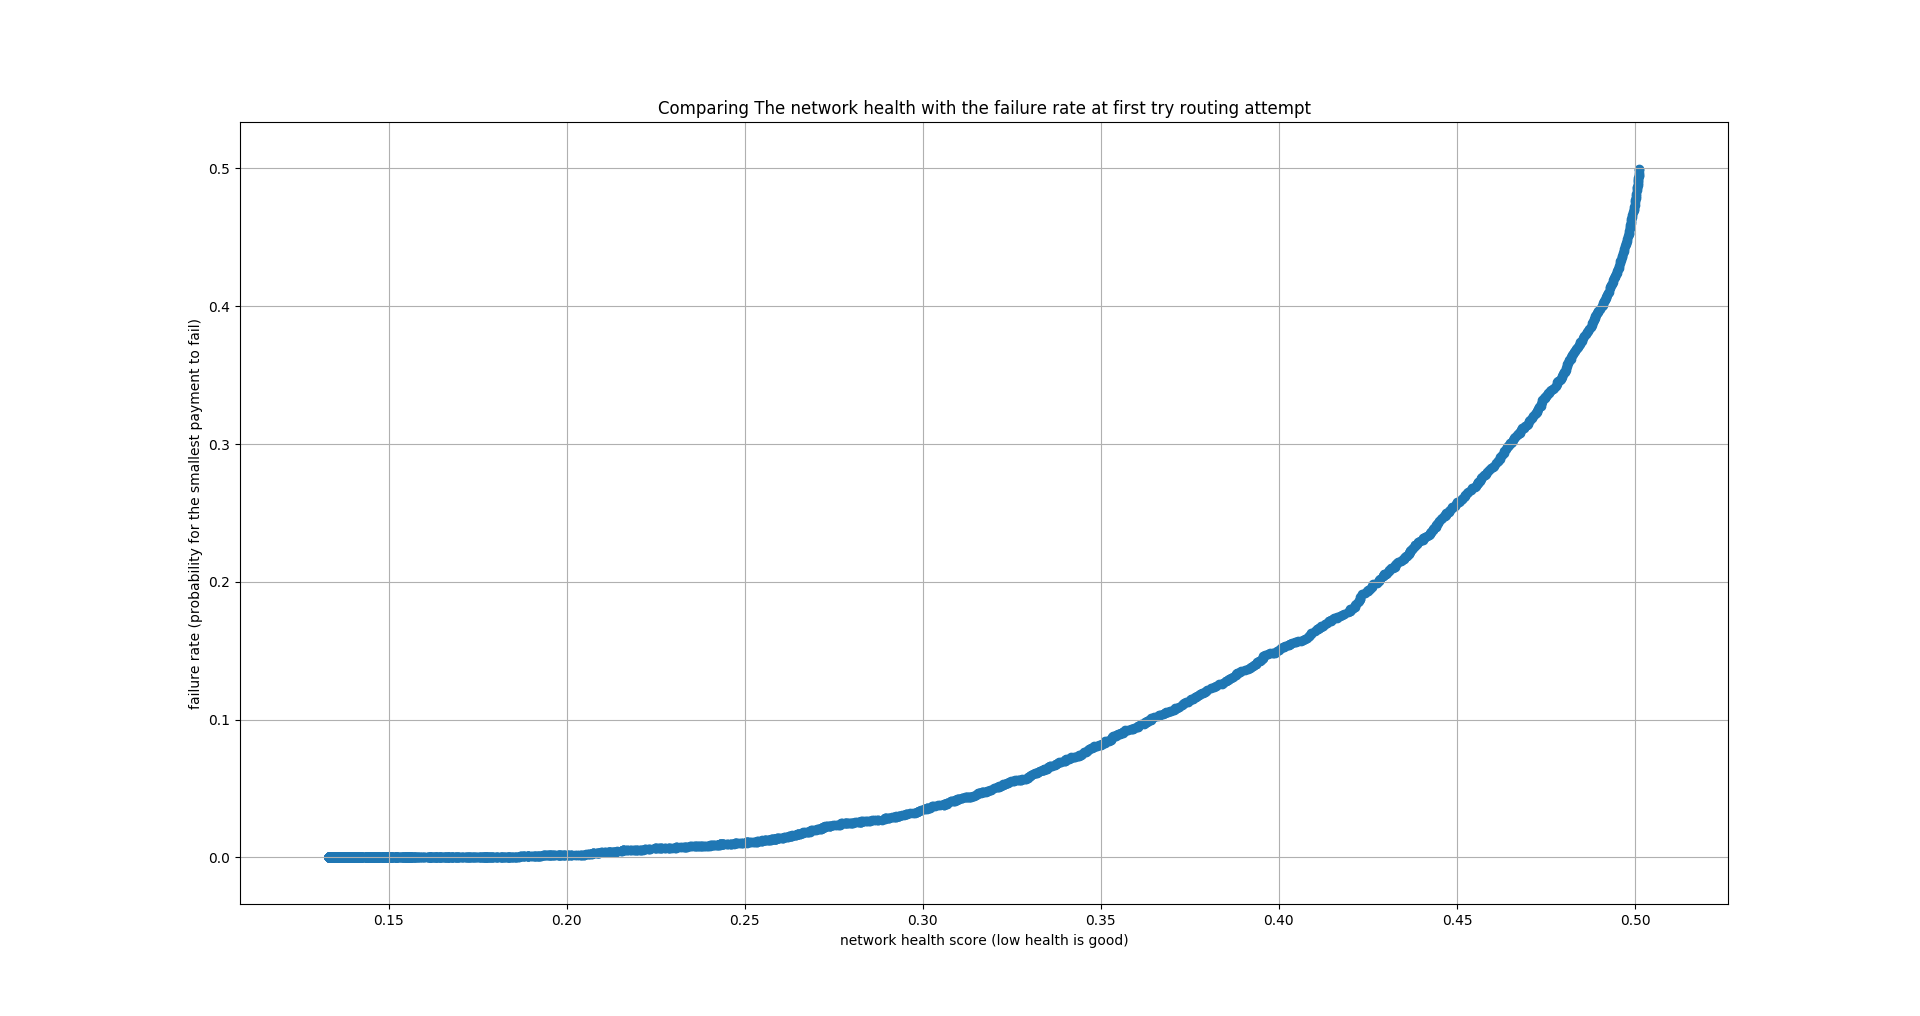
\includegraphics[width=8cm]{code/results/routabilityTest/health vs payment rate.png}
 \caption{For every step of the simulation the health of the network is plotted against the probability for a random payment of the smallest possible amount to fail.}
 \label{fig:healthVsFailurerate}
\end{figure}

In \cref{fig:healthVsFailurerate} we compare our defined health score with the failure rate of payments.
We can see that better (lower) health scores yield a lower failure rate for payments.
The failure rate is measured by attempting a payment between all pairs of nodes and counting the relative amount of payments that cannot be routed on the first selected path from the payment channel network.
We calculate the failure rate and the health score after every simulation step and plot the points as a scatter plot.
This result confirms the dependency of the payment failure and the worse health indicator. It is the first experiment that indicates that the defined health score is semantically correct and well chosen. 

The goal of the second experiment is to check if the overall amounts that can be routed increase with better (lower) health scores.

\begin{figure}
 \centering
 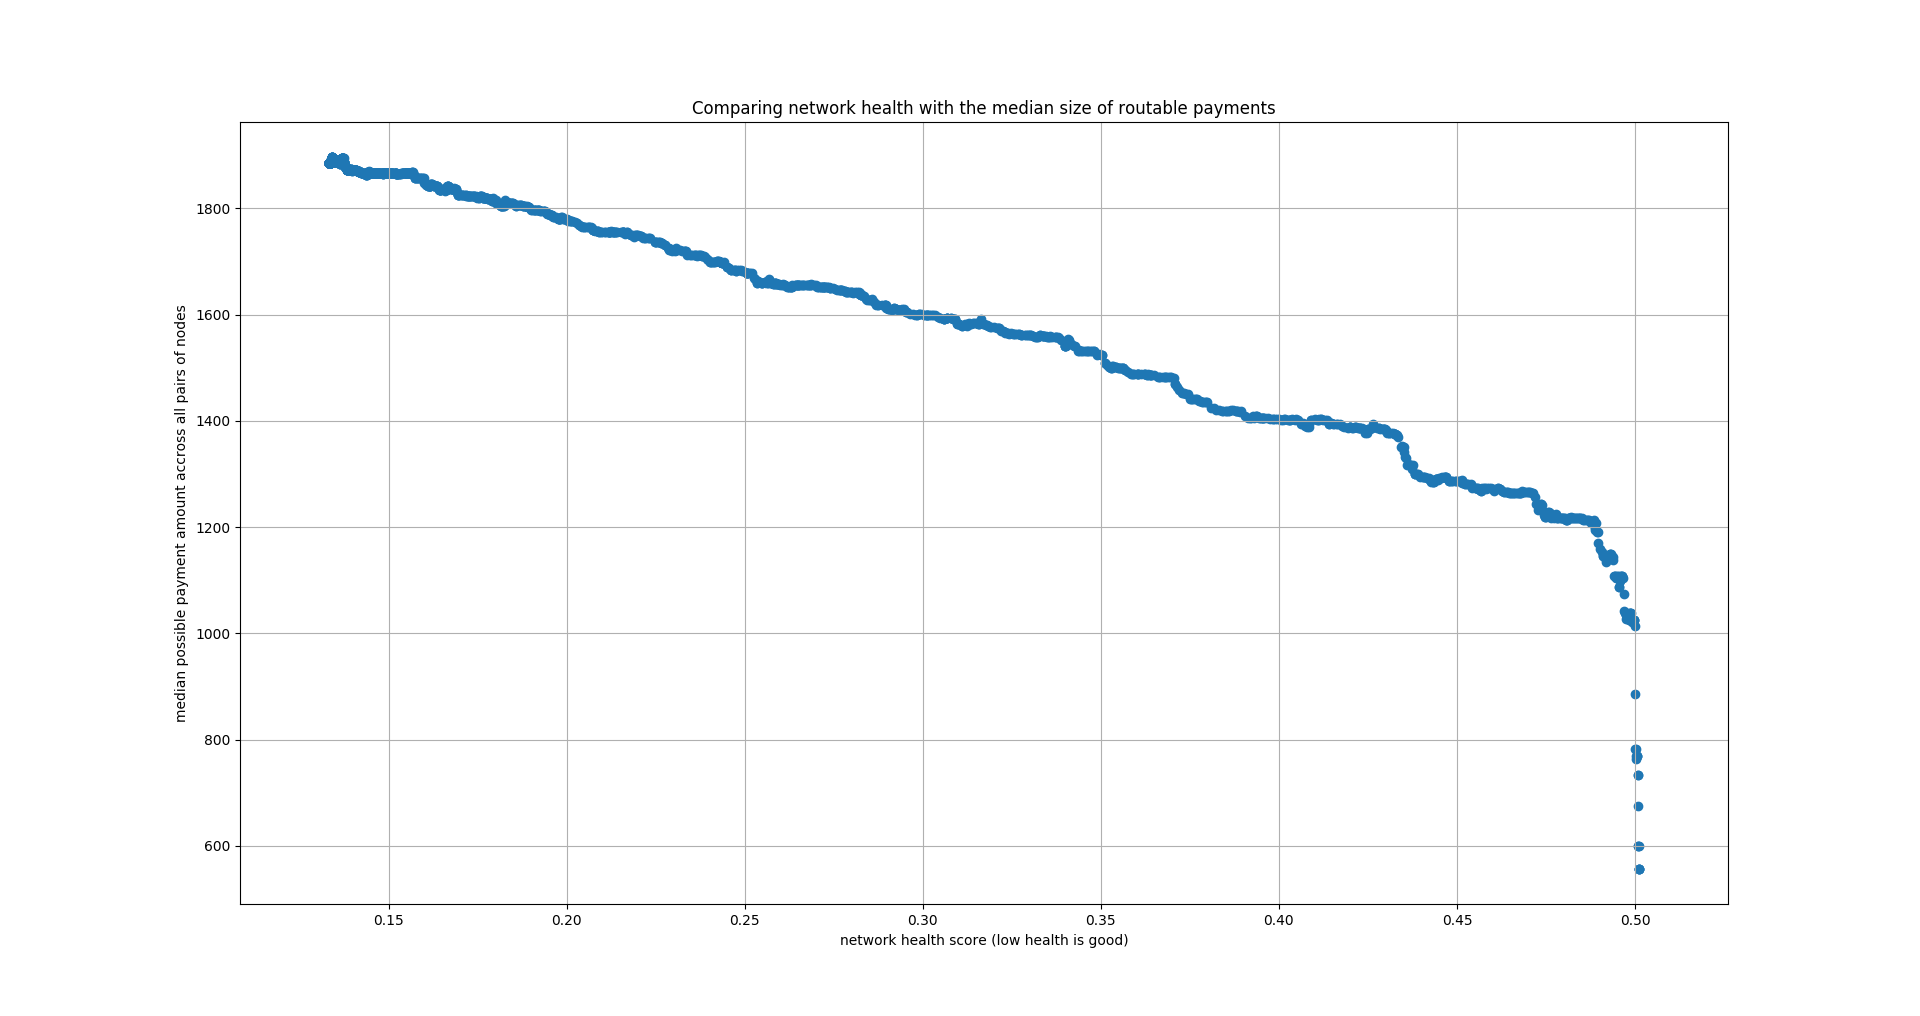
\includegraphics[width=8cm]{code/results/routabilityTest/health vs payment amt.png}
 \caption{For every step of the simulation the health of the network is plotted against the median value of payments that can be fulfilled. Note that failed payments are part of the statistics and counted as payments which can send $0$ satoshi.}
 \label{fig:healthVsPayment}
\end{figure}

In \cref{fig:healthVsPayment} we compare the health score with the median payment amount.
The median payment amount is computed as follows.
First all pair of shortest paths are computed.
We then look at the amount that could actually be forwarded through each path.
Finally we take the median of those amounts.
This means that at least $50\%$ of payment pairs are able to forward this amount.
The higher this amount is the higher payments are supported by the network.
We see a nice negative correlation between the health score and the median routable payment amount.
This suggests that a healthier network is statistically able to route higher payment amounts on the first try.
This is particularly important as privacy aware payment channel networks use source based onion routing and technically have to guess a path. When those initially guessed paths provide a low failure rate with high payment amounts there are considerable benefits for the overall functioning of the payment network. 
The user experience is improved, the payment delays are lowered, and the amount of messaging and coordination is minimised. 

\begin{figure}
 \centering
 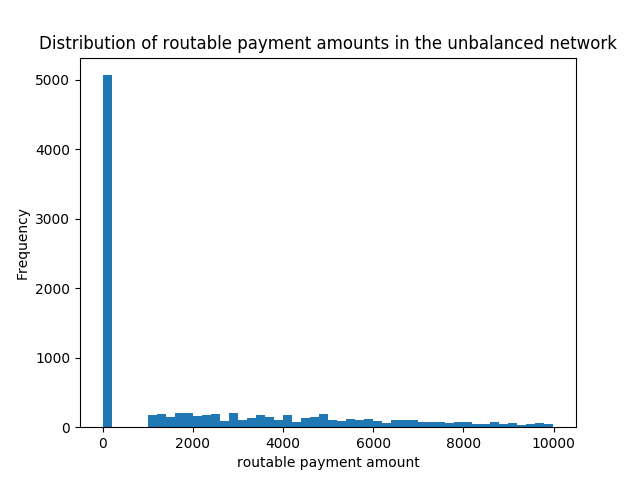
\includegraphics[width=8cm]{code/results/routabilityTest/paymentamtUnbalanced.png}
 \caption{The initial distribution of maximum payment amounts that are possible to be paid on the first routing attempt between all pairs of nodes in the network.}
 \label{fig:paymentUnbalanced}
\end{figure}

\begin{figure}
 \centering
 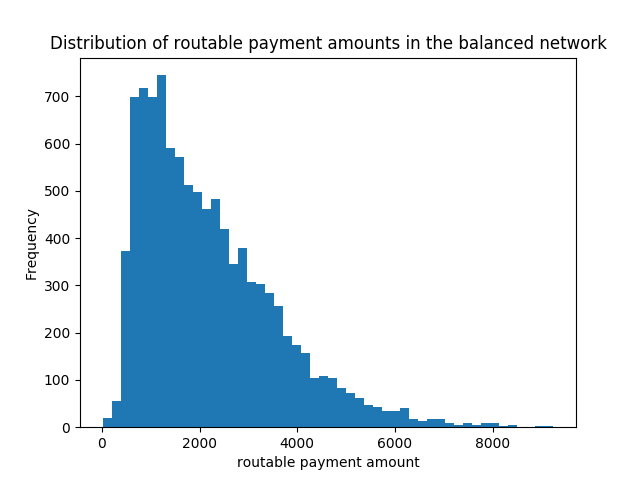
\includegraphics[width=8cm]{code/results/routabilityTest/paymentamtBalanced.png}
 \caption{The final distribution of maximum payment amounts that are possible to be paid on the first routing attempt between all pairs of nodes in the network after the health improving algorithm has converged into a local minimum.}
 \label{fig:paymentBalanced}
\end{figure}

To demonstrate that the median actually makes sense we depict the distribution of possible payment amounts between all pairs of nodes on the unbalanced network which we used as an input for the algorithm in \cref{fig:paymentUnbalanced} and also the distribution of possible. payment amounts on the balanced network after the algorithm has been executed successfully in \cref{fig:paymentBalanced}.

Finally, we have tested, from a statistical point of view, a validity of computing the health as the average of the local health coefficients.
To test that, we verified if the local health coefficients $\nu_u$ for all $u \in N$ follow a normal distribution. This has been successfully confirmed with the D'Agostino normallity test~ß\cite{d1971omnibus}.
This test achieved a p-value of $0.027$ on the balanced network.
One can see in \cref{fig:giniStart} and \cref{fig:giniEnd} how the distribution of local health coefficients looks before and after rebalancing the network. We can see that, on average, the mean of the distribution is being decreased. This is to be expected. 

\begin{figure}
 \centering
 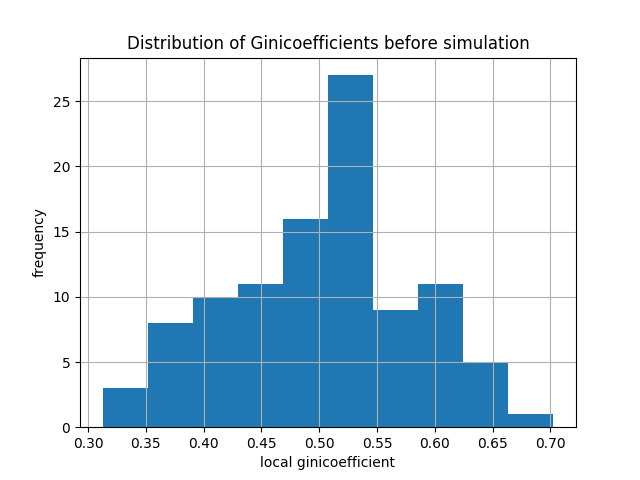
\includegraphics[width=7cm]{code/results/routabilityTest/1574847007_ginicoefficients_start.png}
 \caption{The distribution of Gini-coefficients (local health coefficients) in the unbalanced random network before the simulation started.}
 \label{fig:giniStart}
\end{figure}ß
\begin{figure}
 \centering
 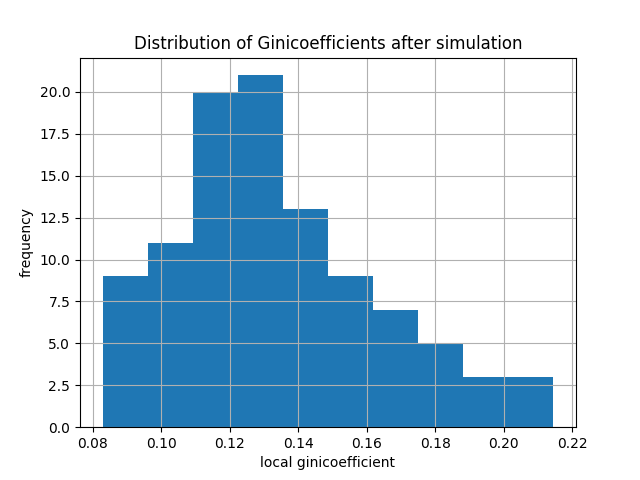
\includegraphics[width=7cm]{code/results/routabilityTest/1574847007_ginicoefficients_end.png}
 \caption{Distribution of Gini-coefficients (local health coefficients) for all nodes in the random network after the health improvement algorithm successfully executed.}
 \label{fig:giniEnd}
\end{figure}


%show (compute!) histograph of the unbalanced and balanced network of payment amounts to make more sense of the median measure
% actually it would be nice to do a kolmogorov smirnof test on distributions by comparing the L_1 norm of the CDFs


% =======================================================================

\section{Conclusion and Discussion}\label{sec:conclusion}
Our experiments support the assumption that payments along an arbitrary or randomly chosen path have a higher successrate if the network is rather balanced.
As privacy aware payment channel networks use source based pathfinding without knowing the constraints of the channels along an attempted path the liklihood of conducting a successfull payment with few appempts becomes considerably higher in a balanced network.
Our results show that nodes do not need to strive for $\nu_u = 0.5$ and perfect local balance of their channels in order to produce a well balanced network with a high successrate of random payments.
Instead it is sufficient for the overall network to be balanced if every node tries to opimize their channel balance coefficients be rather equal. 
This can be achieved by optimizing for a low Ginicoefficient of the channel balance coefficients by making circular rebalancing payments.
In particular we analyzed that the definition of the network imbalance metric as the average of the nodes imbalance metrics is statistically well defined on our test data.
In particular we showed that one could call a payment channel network healthy if the imbalance of the network is low.

In a similar way as internet routers collaboratevly solve the path finding problem by exchanging routing tables we furthermore suggest for the network to work collaboratively towards achieving a good balanceby locally sharing routing hints and allowing for fee free rebalancing operations if everyone along the path benefits from the operation. 
As balances of channels in the friend of a friend network can easily be probed it seems plausible in privacy aware payment channel networks to include a communication protocol with which a node signal their partners that it wants to rebalance a certain channel with a certain amount.
We think that that our suggestion for sharing channels need a rebalancing operation does not reveal more information as can currently be collected with probing attacks anyway.

\section{Future Work}\label{sec:future}
We empirically verified that the health measure increases the overall ability of network participants to route payments on random paths.
However the health measure has some edge cases in which it is breaking with the intuitive semantics a person would have.
Consider for example a node that opens $d$ channels and has all the funds on its side.
In that case the local channel coefficients $\zeta_{(u,v_1)},\dots,\zeta_{(u,v_d)}$ would all take the value of $1$ resulting in $G_0 = 0$ meaning this node is in perfect health.
From a network perspective this node can neither forward any payments can it participat in rebalancing operations.
If the overall topology changes by either $u$ making a payment or another node opening a channel with $u$ this situation would be resolved.
Thus a future work in the direction of autopilots and channel management might include to not only optimize ones node for a low value of $G_u$ but also to optimize towards $\nu_u = 0.5$ or to find out what node balance coefficients would be preferable for node operator with different needs.

In a similar sense it might be interesting to study how nodes could define their local health in different ways and what would happen with the greedy algorithm if different health definitions are followed by nodes.
For example routing nodes or liquidity providers might very well want to have high values of $\zeta$ on some of their channels where as they might be willing to accept low values for $\zeta$ on other channels.
In a similar way merchants will probably prefer many channels with low values of $\zeta$.
The algorithm could very well be exchanged to a version in which nodes decide their own health metric.
Along that line one could ask how the heuristic performes if only a fraction of nodes participate in the sharing of rebalancing hints and fee free rebalancing protocol.

As the simulation was alrady consuming a lot of computational resources we did not check if the algorithm greedy heuristic ist stable under concurrent payments and rebalancing operations taking place.
While the design of the lightning network with setting up htlcs which are locked from the balance at that point anyway suggests that this is not a problem it woul still be nice to see this tested.
In the real world scenario an oscillating algorithm seems to be of little use. 

In section \ref{sec:lnchanges} we have mentioned that besides the communication protocol to share informations about channels there needs to be a transport mechanism for fee free circular payments.
Obviously the onions could not be reused as a node might steal routing fees and hide them as a rebalancing request.
This paper did not discuss the crypotgraphic protocols necessary to ensure that a proovably fee free rebalancing operation can be executed.
While approaches for blockchains with more expressive scripting languages exist \cite{khalil2017revive} we leave it as a future work to provide a cryptographic protocol to be able to fulfill these requests in bitcoin.
While we tested the algorithm and observed its rather quick convergence it might be interesting to study how it adapts if the topology changes in real time due to opening or closing channels as well as a reallocation of funds due to payments that are taking place.

\section{Acknolegements}\label{sec:ack}
We thank xyz...


\bibliography{lightningNetworkHealth}
\bibliographystyle{plain}

\end {document}
